\documentclass[12pt]{article}
\usepackage{amsmath} % AMS Math Package
\usepackage{bm}
\usepackage{amsthm} % Theorem Formatting
\usepackage{amssymb}    % Math symbols such as \mathbb
\usepackage{graphicx} % Allows for eps images
\usepackage[dvips,letterpaper,margin=1in,bottom=0.7in]{geometry}
\usepackage{tensor}
\usepackage{amsmath}
\usepackage{siunitx}
\usepackage{physics}
\usepackage{amsmath, amssymb, graphics, setspace}
\usepackage{listings}
\usepackage{color}

\definecolor{dkgreen}{rgb}{0,0.6,0}
\definecolor{gray}{rgb}{0.5,0.5,0.5}
\definecolor{mauve}{rgb}{0.58,0,0.82}

\lstset{frame=tb,
  language=Java,
  aboveskip=3mm,
  belowskip=3mm,
  showstringspaces=false,
  columns=flexible,
  basicstyle={\small\ttfamily},
  numbers=none,
  numberstyle=\tiny\color{gray},
  keywordstyle=\color{blue},
  commentstyle=\color{dkgreen},
  stringstyle=\color{mauve},
  breaklines=true,
  breakatwhitespace=true,
  tabsize=3
}

\newcommand{\mathsym}[1]{{}}
\newcommand{\unicode}[1]{{}}

\newcounter{mathematicapage}

\newtheorem{p}{Problem}
\usepackage{cancel}
\newtheorem*{lem}{Lemma}
\theoremstyle{definition}
\newtheorem*{dfn}{Definition}
 \newenvironment{s}{%\small%
        \begin{trivlist} \item \textbf{Solution}. }{%
            \hspace*{\fill} $\blacksquare$\end{trivlist}}%

\makeatletter
% we use \prefix@<level> only if it is defined
\renewcommand{\@seccntformat}[1]{%
  \ifcsname prefix@#1\endcsname
    \csname prefix@#1\endcsname
  \else
    \csname the#1\endcsname\quad
  \fi}
% define \prefix@section
\newcommand\prefix@section{}
\newcommand{\prefix@subsection}{}
\newcommand{\prefix@subsubsection}{\thesubsubsection\ - }
\renewcommand{\thesubsection}{\arabic{subsection}}
\makeatother

\begin{document}

 {\noindent\Huge\bf  \\[0.5\baselineskip] {\fontfamily{cmr}\selectfont  Project 2}         }\\[2\baselineskip] % Title
{ {\bf \fontfamily{cmr}\selectfont Quantum Mechanics}\\ {\textit{\fontfamily{cmr}\selectfont     \today}}}~~~~~~~~~~~~~~~~~~~~~~~~~~~~~~~~~~~~~~~~~~~~~~~~~~~~~~~~~~~~~~~~~~~~~~~~~~~~~    {\large \textsc{C Seitz}
\\[1.4\baselineskip] 

\section{Part 1}


\begin{figure}
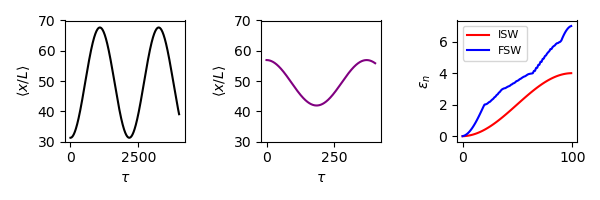
\includegraphics[scale=1.25]{Figure_1.png}
\centering
\caption{Expectation values of position as a function of time for the infinite (left) and finite (right) square well}
\end{figure}

We can work in a coordinate system centered on zero, and write

\begin{align*}
\langle x \rangle &= \sum_{a'}\sum_{a''}c_{a'}^{*}c_{a''}\bra{a'}x\ket{a''}\exp\left(\frac{-i(E_{a''}-E_{a'})t}{\hbar}\right)\\
&= \frac{1}{2}\left(\bra{0}x\ket{1}\exp\left(\frac{-i(E_{1}-E_{0})t}{\hbar}\right) + \bra{1}x\ket{0}\exp\left(\frac{-i(E_{0}-E_{1})t}{\hbar}\right)\right)\\
&= \beta \cos(\omega t)
\end{align*}

where $\beta = \bra{0}x\ket{1} = \bra{1}x\ket{0}$ (because $x$ is Hermitian) and $\omega = (E_1-E_0)/\hbar$. The angular frequency is higher for the finite square well because there is a large energy gap between the first excited state and the ground state (see the differential in the eigenvalue spectrum in Figure 1c).

\section{Part 2}

We are using the time-dependent Hamiltonian

\begin{align*}
H(x,t) = H_{0}(x) + \lambda(1-e^{-t/\tau})V(x)
\end{align*}

where $V(x)$ is the finite square well potential. We are assuming that $\tau\rightarrow\infty$ so the potentially turns on exactly at $t=0$, giving a constant perturbation. Notice that $V$ is going to be needed in energy basis, so we will need to transform $V$ using the unitary operator (the $\ket{i}$ basis to the $\ket{\epsilon_{n}}$ basis).


\noindent \textbf{(H)} We are after $P_{n}(t) = |c_{n}^{(1)}(t)|^{2}$ for $n=1,2,3$. In the text, we are given

\begin{align*}
c_{n}^{(1)}(t) &= -\frac{i}{\hbar}V_{ni}\int_{0}^{t}e^{i\omega_{ni}t}dt\\
&= \frac{V_{ni}}{E_{n}-E_{i}}(1-e^{i\omega_{ni}t})
\end{align*}

where $V_{ni} = \bra{n}V\ket{i}$. 
\begin{align*}
|c_{n}^{(1)}(t)|^{2} &= \frac{4|V_{ni}|^{2}}{|E_{n}-E_{i}|^{2}}\sin^{2}\left(\frac{(E_{n}-E_{i})t}{2\hbar}\right)
\end{align*}


\clearpage
\begin{lstlisting}


\end{lstlisting}

\end{document}